% BARCS student guide for grades 7-9.
% Written to the rules of ASD-STE100 Simplified Technical English:
% short sentences, active voice, present tense, one idea per sentence,
% one meaning per word, and every symbol defined before use.
% Build: pdflatex barcs_student_guide.tex (run twice for the contents list).
\documentclass[12pt]{article}

\usepackage[margin=1in]{geometry}
\usepackage[T1]{fontenc}
\usepackage{lmodern}
\usepackage{amsmath,amssymb}
\usepackage{booktabs}
\usepackage{array}
\usepackage{enumitem}
\usepackage[most]{tcolorbox}
\usepackage{xcolor}
\usepackage{tikz}
\usetikzlibrary{arrows.meta,positioning}
\usepackage[hidelinks]{hyperref}

\definecolor{barcsblue}{HTML}{0072B2}
\definecolor{barcsgreen}{HTML}{009E73}
\definecolor{barcsorange}{HTML}{D55E00}

\newtcolorbox{symbols}{colback=barcsblue!5,colframe=barcsblue,
  fonttitle=\bfseries,title=What the symbols mean,boxrule=0.6pt,arc=2pt}
\newtcolorbox{worked}[1][]{colback=barcsgreen!5,colframe=barcsgreen!80!black,
  fonttitle=\bfseries,title=Worked example#1,boxrule=0.6pt,arc=2pt}
\newtcolorbox{remember}{colback=barcsorange!5,colframe=barcsorange,
  fonttitle=\bfseries,title=Remember,boxrule=0.6pt,arc=2pt}

\newlist{choices}{enumerate}{1}
\setlist[choices]{label=(\Alph*),leftmargin=2.2em,itemsep=1pt,topsep=2pt}
\setlist{itemsep=2pt}

\setlength{\parskip}{6pt}
\setlength{\parindent}{0pt}

\title{\textbf{How BARCS Finds Important Genes}\\[6pt]
\large A student guide with worked examples and a quiz}
\author{Prepared for Hyun-Hwan Jeong and Kyu-Won Lee}
\date{BARCS version 0.2.1 \quad$\cdot$\quad Reading level: grades 7 to 9}

\begin{document}
\maketitle

\begin{center}
\begin{minipage}{0.85\textwidth}
\small
\textbf{About this guide.} This guide explains how the BARCS computer
program works. You need only arithmetic, fractions, percents, powers and
square roots. The guide teaches logarithms when it uses them. Each section
uses the same small set of numbers, so you can follow every step. The guide
uses the writing rules of ASD-STE100 Simplified Technical English.
\end{minipage}
\end{center}

\tableofcontents
\newpage

%=====================================================================
\section{The experiment: a CRISPR screen}
%=====================================================================

Each cell in your body has about 20{,}000 genes. A gene is a set of
instructions. Scientists want to know which genes a cell needs, for example
to survive a cancer drug.

A \textbf{CRISPR screen} tests thousands of genes at the same time. It works
in four steps:

\begin{enumerate}
\item Scientists make a \textbf{library} of short pieces of RNA, called
  \textbf{guides}. Each guide switches off one gene.
\item They put one guide into each cell. Now each cell has one gene switched
  off.
\item They grow the cells. Some cells grow under normal conditions
  (\textbf{control}). Other cells grow with a drug (\textbf{drug}).
\item A sequencing machine reads the guides in each group. The machine
  counts how many times it reads each guide. This number is a
  \textbf{read count}.
\end{enumerate}

If cells need a gene to survive the drug, the cells that lose that gene die.
Their guide becomes rare in the drug group. So the guide count goes down.

\begin{remember}
BARCS does not look at cells directly. It looks at read counts. A guide that
becomes rare tells us that its gene is important.
\end{remember}

Scientists repeat each group more than one time. Each repeat is a
\textbf{replicate}. Each sample that the machine reads is a \textbf{library}.
In this guide, we use four libraries: two control replicates and two drug
replicates.

%=====================================================================
\section{The data}
%=====================================================================

The machine gives two numbers for each library:

\begin{itemize}
\item the read count of our guide, and
\item the total read count of all guides in that library.
\end{itemize}

Table~\ref{tab:data} shows the data for one guide. We use these numbers in
all sections of this guide.

\begin{table}[h]
\centering
\caption{Read counts for one guide in four libraries.}
\label{tab:data}
\begin{tabular}{lcrr}
\toprule
Library & Group & Guide count $K$ & Total count $N$\\
\midrule
1 & control & 180 & 1{,}000{,}000\\
2 & control & 240 & 1{,}200{,}000\\
3 & drug    & 120 & 1{,}000{,}000\\
4 & drug    &  80 &   800{,}000\\
\bottomrule
\end{tabular}
\end{table}

\begin{symbols}
\begin{tabular}{@{}l p{0.78\linewidth}@{}}
$K$ & The read count of one guide in one library. Library~1 has $K=180$.\\
$N$ & The total read count of all guides in one library. Library~1 has
      $N=1{,}000{,}000$.\\
$i$ & The library number (1, 2, 3 or 4). We write $K_i$ for the count in
      library $i$. So $K_2=240$.\\
\end{tabular}
\end{symbols}

\begin{remember}
Always record $N$ before you remove any guides from the table. If you remove
guides first, the totals become wrong. Then all the later numbers become
wrong too.
\end{remember}

%=====================================================================
\section{Step 1: Turn counts into proportions}
%=====================================================================

Library~2 has more reads than library~1 because the machine read it more.
So we cannot compare raw counts. We divide each count by its library total.
The result is a \textbf{proportion}:
\[
p = \frac{K}{N}.
\]

Proportions are very small numbers. So we multiply by one million. The
result is the count \textbf{per million} reads.

\begin{worked}[ 1: proportions]
\begin{tabular}{@{}lll@{}}
Library 1: & $p = 180 \div 1{,}000{,}000 = 0.000180$ & $= 180$ per million\\
Library 2: & $p = 240 \div 1{,}200{,}000 = 0.000200$ & $= 200$ per million\\
Library 3: & $p = 120 \div 1{,}000{,}000 = 0.000120$ & $= 120$ per million\\
Library 4: & $p = \phantom{0}80 \div \phantom{0,}800{,}000 = 0.000100$ & $= 100$ per million\\
\end{tabular}

\smallskip
The two control libraries give 180 and 200 per million. The two drug
libraries give 120 and 100 per million. The guide is less common with the
drug.
\end{worked}

\begin{symbols}
\begin{tabular}{@{}l p{0.78\linewidth}@{}}
$p$ & The proportion of all reads that belong to the guide. It is always
      between 0 and 1.\\
\end{tabular}
\end{symbols}

%=====================================================================
\section{Step 2: Compare the groups with a fold change}
%=====================================================================

We want one number that tells how much the guide changes. First, we combine
the replicates of each group. We add their counts and add their totals:

\[
p_{\text{control}} = \frac{180+240}{1{,}000{,}000+1{,}200{,}000}
 = \frac{420}{2{,}200{,}000} = 0.000191 \;(191 \text{ per million}),
\]
\[
p_{\text{drug}} = \frac{120+80}{1{,}000{,}000+800{,}000}
 = \frac{200}{1{,}800{,}000} = 0.000111 \;(111 \text{ per million}).
\]

The \textbf{fold change} is the drug proportion divided by the control
proportion:
\[
\text{fold change} = \frac{p_{\text{drug}}}{p_{\text{control}}}
 = \frac{0.000111}{0.000191} = 0.58.
\]

A fold change of 0.58 means that the guide keeps only 58\% of its control
level. It loses 42\%.

\begin{remember}
\begin{itemize}[leftmargin=1.2em]
\item Fold change $= 1$: no change.
\item Fold change $< 1$: the guide becomes rarer. Cells may need this gene.
\item Fold change $> 1$: the guide becomes more common. Losing this gene
  may help the cells.
\end{itemize}
\end{remember}

\subsection{Logarithms make changes symmetric}

A fold change of 2 means ``double''. A fold change of 0.5 means ``half''.
These changes have the same size, but the numbers 2 and 0.5 do not look
equal. A \textbf{logarithm} fixes this problem.

The \textbf{base-2 logarithm}, $\log_2$, tells how many times you double.
\begin{center}
\begin{tabular}{lccccc}
\toprule
Fold change & 0.25 & 0.5 & 1 & 2 & 4\\
$\log_2$(fold change) & $-2$ & $-1$ & 0 & 1 & 2\\
\bottomrule
\end{tabular}
\end{center}
Now ``double'' is $+1$ and ``half'' is $-1$. The sizes look equal.

\begin{worked}[ 2: log fold change]
Our fold change is 0.58. It is between 0.5 and 1. So $\log_2(0.58)$ is
between $-1$ and 0. A calculator gives $\log_2(0.58) = -0.78$.

The guide drops by 0.78 ``halvings''.
\end{worked}

BARCS uses the \textbf{natural logarithm}, $\ln$. It counts powers of the
number $e = 2.718\ldots$ instead of powers of 2. The idea is the same. To
change back from $\ln$, you raise $e$ to that power: if $\ln(x) = b$, then
$x = e^{b}$. For our guide, $\ln(0.58) = -0.54$.

%=====================================================================
\section{Step 3: Odds and log-odds}
%=====================================================================

BARCS works with \textbf{odds} instead of proportions. The odds compare the
reads that belong to the guide with the reads that do not:
\[
\text{odds} = \frac{p}{1-p}.
\]
The \textbf{log-odds} is the natural logarithm of the odds:
\[
\text{log-odds} = \ln\!\left(\frac{p}{1-p}\right).
\]

\begin{worked}[ 3: odds and log-odds]
Control: $p = 0.000191$. So
$\text{odds} = 0.000191 \div 0.999809 = 0.000191$.

The odds and the proportion are almost equal. This is true for all small
proportions, because $1-p$ is almost 1.

Log-odds for control: $\ln(0.000191) = -8.56$.\\
Log-odds for drug: $\ln(0.000111) = -9.10$.\\
Difference: $-9.10 - (-8.56) = -0.54$.

The difference of the log-odds is $-0.54$. This is the same as
$\ln(\text{fold change})$ from Step~2.
\end{worked}

\begin{remember}
For guides, a difference in log-odds is almost exactly the natural log of
the fold change. So you can read BARCS results as log fold changes.
\end{remember}

Why use log-odds at all? A proportion must stay between 0 and 1. A log-odds
can be any number, positive or negative. This property lets BARCS add
effects together safely, as Step~5 shows.

%=====================================================================
\section{Step 4: Two kinds of noise}
%=====================================================================

The two control libraries gave 180 and 200 per million. They are not equal.
Replicates always differ a little. We call this difference
\textbf{noise}. BARCS must know how big the noise is. Then it can tell a
real change from a chance change.

Guide counts have two kinds of noise:

\begin{enumerate}
\item \textbf{Counting noise.} The machine reads a random sample of all
  the guides. Think of a bag with a million marbles. You take out a handful.
  You do not get exactly the same number of red marbles each time.
\item \textbf{Biological noise.} Each replicate is a different group of
  living cells. The cells grow a little differently each time.
\end{enumerate}

BARCS measures the size of the noise with the \textbf{variance}. The
variance is the average squared distance of a value from its expected
value. The \textbf{standard deviation} is the square root of the variance.
It is the typical distance in the same units as the counts.

BARCS uses this formula for the variance of a guide count:
\[
\text{variance} = \underbrace{N\,\mu\,(1-\mu)}_{\text{counting noise}}
 \times \underbrace{\bigl(1 + (N-1)\,\rho\bigr)}_{\text{extra biological noise}}.
\]

\begin{symbols}
\begin{tabular}{@{}l p{0.78\linewidth}@{}}
$\mu$ & ``mu''. The true proportion of the guide that we expect. For the
        control group, our best value is $\mu = 0.000191$.\\
$N$ & The library total, as before.\\
$\rho$ & ``rho''. A number that measures the biological noise. If
         $\rho = 0$, only counting noise exists. A bigger $\rho$ means more
         biological noise.\\
\end{tabular}
\end{symbols}

\begin{worked}[ 4: variance]
Use $N = 1{,}000{,}000$ and $\mu = 0.000191$. For our guide, BARCS
estimates $\rho = 0.000000386$.

\textbf{Counting noise:}
$N\mu(1-\mu) = 1{,}000{,}000 \times 0.000191 \times 0.999809 = 191$.

\textbf{Extra factor:}
$1 + (N-1)\rho = 1 + 999{,}999 \times 0.000000386 = 1.39$.

\textbf{Total variance:} $191 \times 1.39 = 265$.

\textbf{Standard deviation:} $\sqrt{265} = 16.3$ reads.

So a count of about 191 normally moves up or down by about 16. Biological
noise adds 39\% to the counting noise.
\end{worked}

\begin{remember}
Look at the extra factor $1 + (N-1)\rho$. It contains $N$. When the machine
reads more, $N$ grows, and the factor grows too. So more reading does not
remove biological noise. Only more replicates help with biological noise.
\end{remember}

%=====================================================================
\section{Step 5: The design matrix}
%=====================================================================

A \textbf{model} is a rule that predicts a value. BARCS predicts the
log-odds of a guide in each library. The model needs to know which group
each library belongs to. BARCS gets this information from the
\textbf{design matrix}.

\subsection{What a design matrix is}

A design matrix is a table of numbers. It has:
\begin{itemize}
\item one \textbf{row} for each library, and
\item one \textbf{column} for each $\beta$ value in the model.
\end{itemize}
We write the design matrix with the letter $X$.

For our four libraries, the model has two $\beta$ values. So $X$ has four
rows and two columns:

\begin{center}
\begin{tabular}{lc|cc}
\toprule
Library & Group & Column 1: ``intercept'' & Column 2: ``drug''\\
\midrule
1 & control & 1 & 0\\
2 & control & 1 & 0\\
3 & drug    & 1 & 1\\
4 & drug    & 1 & 1\\
\bottomrule
\end{tabular}
\end{center}

\begin{symbols}
\begin{tabular}{@{}l p{0.74\linewidth}@{}}
$X$ & The design matrix. One row for each library, one column for each
      $\beta$.\\
Intercept & A column of 1s. It belongs to $\beta_0$, the starting level.
      Every library gets the starting level.\\
Drug & A column that is 1 for a drug library and 0 for a control library.
      It belongs to $\beta_1$, the effect of the drug.\\
$\beta_0$ & ``beta zero''. The log-odds of the guide in the control group.\\
$\beta_1$ & ``beta one''. The change in log-odds from control to drug. This
      is the \textbf{effect}. It is the most important number.\\
\end{tabular}
\end{symbols}

\subsection{From the design matrix to a prediction}

To get the prediction for one library, take the row of that library. Multiply
each number in the row by its $\beta$. Then add the products:
\[
\text{predicted log-odds} = (\text{column 1}) \times \beta_0 +
(\text{column 2}) \times \beta_1 .
\]
This calculation is a \textbf{matrix multiplication}. You do it one row at
a time. We call the predicted log-odds $\eta$ (``eta'').

\begin{worked}[ 5: predictions from the design matrix]
BARCS finds $\beta_0 = -8.565$ and $\beta_1 = -0.542$ (Step~6 shows how).

\begin{tabular}{@{}lll@{}}
Library 1 (row 1, 0): & $1 \times (-8.565) + 0 \times (-0.542)$ & $= -8.565$\\
Library 2 (row 1, 0): & $1 \times (-8.565) + 0 \times (-0.542)$ & $= -8.565$\\
Library 3 (row 1, 1): & $1 \times (-8.565) + 1 \times (-0.542)$ & $= -9.107$\\
Library 4 (row 1, 1): & $1 \times (-8.565) + 1 \times (-0.542)$ & $= -9.107$\\
\end{tabular}

\smallskip
The control libraries get $\beta_0$ only. The drug libraries get
$\beta_0 + \beta_1$. So $\beta_1$ is the difference between the groups.
\end{worked}

\subsection{From log-odds back to counts}

A prediction in log-odds is hard to read. So we change it back into a
proportion, and then into a count. The rule is:
\[
\mu = \frac{e^{\eta}}{1 + e^{\eta}}, \qquad
\text{expected count} = N \times \mu .
\]
This rule undoes the log-odds of Step~3.

\begin{worked}[ 6: expected counts]
\textbf{Control libraries} ($\eta = -8.565$):
$e^{-8.565} = 0.000190676$. Then
$\mu = 0.000190676 \div 1.000190676 = 0.000190640$, which is 190.6 per
million.

\textbf{Drug libraries} ($\eta = -9.107$):
$e^{-9.107} = 0.000110840$. Then $\mu = 0.000110827$, which is 110.8 per
million.

\begin{tabular}{@{}lrrrr@{}}
\toprule
Library & $N$ & $\mu$ (per million) & Expected count $N\mu$ & Real count $K$\\
\midrule
1 & 1{,}000{,}000 & 190.6 & 190.6 & 180\\
2 & 1{,}200{,}000 & 190.6 & 228.8 & 240\\
3 & 1{,}000{,}000 & 110.8 & 110.8 & 120\\
4 &   800{,}000 & 110.8 &  88.7 &  80\\
\bottomrule
\end{tabular}

\smallskip
The expected counts are near the real counts. The differences are
$-10.6$, $+11.2$, $+9.2$ and $-8.7$ reads. These differences are the noise.
\end{worked}

\subsection{The reference group}

The control group has 0 in the drug column. So control is the
\textbf{reference group}. The effect $\beta_1$ always compares a group with
the reference group. If you make drug the reference group, $\beta_1$ changes
sign. It becomes $+0.542$. The meaning stays the same.

\subsection{Paired replicates: add a column}

Sometimes the replicates are pairs. For example, replicate~1 of control and
replicate~1 of drug come from the same batch of cells. Then BARCS can remove
the batch difference. You add a column for the batch:

\begin{center}
\begin{tabular}{lcc|ccc}
\toprule
Library & Group & Replicate & Intercept & Replicate 2 & Drug\\
\midrule
1 & control & 1 & 1 & 0 & 0\\
2 & control & 2 & 1 & 1 & 0\\
3 & drug    & 1 & 1 & 0 & 1\\
4 & drug    & 2 & 1 & 1 & 1\\
\bottomrule
\end{tabular}
\end{center}

Now the model has three $\beta$ values: the starting level, the batch
difference and the drug effect. Each new column costs one degree of freedom
(Step~8). With four libraries and three columns, only one degree of freedom
stays.

\begin{worked}[ 7: the paired model for our guide]
BARCS gives the drug effect $\beta = -0.544$ with standard error 0.143.
The effect is almost the same as before ($-0.542$). But the degrees of
freedom drop from 2 to 1. The p-value becomes 0.164 instead of 0.033.

Our two replicates have almost no batch difference ($\beta = 0.005$). So
the extra column costs information and gives nothing back. Add a batch
column only when the replicates really are pairs.
\end{worked}

\subsection{Numbers instead of groups}

A column can also hold a number, for example the day of the experiment.
Suppose that you collect cells on day 0, day 7 and day 14, two libraries
each. You put the day divided by 14 into a column:

\begin{center}
\begin{tabular}{lc|cc}
\toprule
Library & Day & Intercept & Day $\div$ 14\\
\midrule
1, 2 & 0  & 1 & 0\\
3, 4 & 7  & 1 & 0.5\\
5, 6 & 14 & 1 & 1\\
\bottomrule
\end{tabular}
\end{center}

Now $\beta_1$ is the change in log-odds over 14 days. The model draws a
straight line through the three days.

\begin{worked}[ 8: a time course]
Suppose that $\beta_1 = -0.70$.

After 14 days: change $= 1 \times (-0.70) = -0.70$. Fold change
$= e^{-0.70} = 0.50$. The guide drops to half.

After 7 days: change $= 0.5 \times (-0.70) = -0.35$. Fold change
$= e^{-0.35} = 0.70$. The guide drops to 70\%.

The model has 6 libraries and 2 columns. So it has $6 - 2 = 4$ degrees of
freedom.
\end{worked}

\subsection{Two factors and an interaction}

Some experiments change two things. For example, cells can be normal or can
have a second gene switched off (``knockout''). And cells can get no drug or
the drug. This experiment has four groups. The design matrix has four
columns:

\begin{center}
\begin{tabular}{l|cccc}
\toprule
Group & Intercept & Knockout & Drug & Knockout $\times$ Drug\\
\midrule
normal, no drug   & 1 & 0 & 0 & 0\\
knockout, no drug & 1 & 1 & 0 & 0\\
normal, drug      & 1 & 0 & 1 & 0\\
knockout, drug    & 1 & 1 & 1 & 1\\
\bottomrule
\end{tabular}
\end{center}

The last column is the product of the knockout column and the drug column.
It is 1 only when both are 1. Its $\beta$ is the \textbf{interaction}. The
interaction measures the extra change that happens only when both changes
happen together.

\begin{worked}[ 9: reading an interaction]
Suppose that the four $\beta$ values are $-8.5$, $-0.2$, $+0.1$ and
$-0.7$. Multiply each row by the $\beta$ values and add:

\begin{tabular}{@{}ll@{}}
normal, no drug: & $-8.5$\\
knockout, no drug: & $-8.5 + (-0.2) = -8.7$\\
normal, drug: & $-8.5 + 0.1 = -8.4$\\
knockout, drug: & $-8.5 + (-0.2) + 0.1 + (-0.7) = -9.3$\\
\end{tabular}

\smallskip
The knockout alone changes the log-odds by $-0.2$. The drug alone changes it
by $+0.1$. If the two effects only added up, the last group would be
$-8.5 - 0.2 + 0.1 = -8.6$. The real value is $-9.3$. The extra $-0.7$ is the
interaction. The guide drops strongly only when both changes happen.
\end{worked}

\subsection{Comparing two treatments: a contrast}

Suppose an experiment has three groups: control, drug A and drug B. The
design matrix has the columns intercept, drug A and drug B. Then $\beta_A$
compares drug A with control, and $\beta_B$ compares drug B with control. To
compare drug A with drug B, you subtract: $\beta_A - \beta_B$. This
calculation is a \textbf{contrast}. In BARCS, the function
\texttt{bb\_contrast()} calculates it and its test.

For example, if $\beta_A = -0.9$ and $\beta_B = -0.4$, then
$\beta_A - \beta_B = -0.5$. Drug A lowers the guide more than drug B.

\subsection{Rules for a good design matrix}

\begin{enumerate}
\item Make one row for each library, in the same order as the count table.
\item Make one column for each $\beta$ that you want.
\item Keep more rows than columns. The difference is the degrees of
  freedom. Two or more is better than one.
\item Do not let two columns carry the same information. For example,
  suppose that all drug libraries come from batch~2. Suppose also that all
  control libraries come from batch~1. Then the batch column and the drug
  column are equal. BARCS cannot separate the drug effect from the batch
  effect.
\end{enumerate}

\subsection{The design matrix in R}

In R, you describe the design matrix with a \textbf{formula}. The formula
\texttt{\textasciitilde\ group} means ``an intercept and a column for each
group except the reference group''.

The function \texttt{model.matrix()} builds $X$ from the formula:

\begin{center}
\begin{minipage}{0.86\textwidth}
\small
\begin{verbatim}
> data <- data.frame(group = c("control", "control", "drug", "drug"))
> model.matrix(~ group, data)
  (Intercept) groupdrug
1           1         0
2           1         0
3           1         1
4           1         1
\end{verbatim}
\end{minipage}
\end{center}

Then you give the counts, the totals, the formula and the column name to
BARCS:

\begin{center}
\begin{minipage}{0.86\textwidth}
\small
\begin{verbatim}
fit <- bb_screen(counts, data, formula = ~ group,
                 term = "groupdrug", totals = totals)
\end{verbatim}
\end{minipage}
\end{center}

For the paired design, use the formula \texttt{\textasciitilde\ replicate +
group}. For the interaction, use \texttt{\textasciitilde\ knockout * drug}.

%=====================================================================
\section{Step 6: How BARCS finds the best \texorpdfstring{$\beta$}{beta} values}
%=====================================================================

BARCS cannot find $\beta_0$ and $\beta_1$ in one calculation. It uses a loop
of ``guess, check, improve''. The name of this method is
\textbf{iteratively reweighted least squares} (IRLS). Each pass through the
loop is an \textbf{iteration}.

\subsection{The loop}

\begin{enumerate}
\item \textbf{Guess.} Start with the simple log-odds of each group
  (Step~3).
\item \textbf{Predict.} Use the design matrix to predict $\eta$ and $\mu$
  for each library (Step~5).
\item \textbf{Measure the noise.} Find $\rho$ from the differences between
  the real and the expected counts (Step~7).
\item \textbf{Weigh.} Give each library a \textbf{weight}. A library with
  less noise gets a larger weight.
\item \textbf{Correct.} Calculate a corrected value, the \textbf{working
  value}, for each library.
\item \textbf{Improve.} Take a weighted average of the working values in each
  group. These averages give the new $\beta$ values.
\item \textbf{Repeat} from part~2 until the $\beta$ values stop changing.
\end{enumerate}

\subsection{The formulas}

The weight of library $i$ is
\[
w_i = \frac{N_i\,\mu_i\,(1-\mu_i)}{1 + (N_i - 1)\,\rho}.
\]
The top is the counting noise turned upside down. The bottom is the extra
biological noise from Step~4. So more noise gives a smaller weight.

The working value of library $i$ is
\[
\text{working value}_i = \eta_i + \frac{K_i/N_i - \mu_i}{\mu_i\,(1-\mu_i)}.
\]
It is the current prediction $\eta_i$ plus a correction. The correction is
large when the real proportion $K_i/N_i$ is far from the expected proportion
$\mu_i$.

For our design matrix, the new $\beta$ values are weighted averages:
\[
\beta_0 = \frac{w_1\,v_1 + w_2\,v_2}{w_1 + w_2}, \qquad
\beta_0 + \beta_1 = \frac{w_3\,v_3 + w_4\,v_4}{w_3 + w_4},
\]
where $v_i$ is the working value of library $i$. (For other design matrices,
BARCS solves a small set of equations instead. The idea is the same.)

\subsection{Iteration 1 in full}

\begin{worked}[ 10: iteration 1]
\textbf{Guess.} From Step~3, the control log-odds is $-8.563522$ and the
drug log-odds is $-9.104869$. So $\beta_0 = -8.563522$ and
$\beta_1 = -9.104869 - (-8.563522) = -0.541347$.

\textbf{Predict.} The control libraries get $\mu = 0.000190909$. The drug
libraries get $\mu = 0.000111111$.

\textbf{Measure the noise.} Step~7 gives $\rho = 0.0000003841$ for these
predictions.

\textbf{Weigh library 1.}
Top: $1{,}000{,}000 \times 0.000190909 \times 0.999809 = 190.87$.\\
Bottom: $1 + 999{,}999 \times 0.0000003841 = 1.3841$.\\
Weight: $w_1 = 190.87 \div 1.3841 = 137.90$.

\textbf{Correct library 1.}
$K_1/N_1 - \mu_1 = 0.000180 - 0.000190909 = -0.0000109$.\\
$\mu_1(1-\mu_1) = 0.000190873$.\\
Correction: $-0.0000109 \div 0.000190873 = -0.0572$.\\
Working value: $v_1 = -8.5635 + (-0.0572) = -8.6207$.

The same calculations for all four libraries give:

\begin{tabular}{@{}lrrr@{}}
\toprule
Library & Weight $w_i$ & Working value $v_i$ & $w_i \times v_i$\\
\midrule
1 (control) & 137.905 & $-8.62068$ & $-1188.84$\\
2 (control) & 156.785 & $-8.51589$ & $-1335.16$\\
3 (drug)    &  80.269 & $-9.02486$ &  $-724.42$\\
4 (drug)    &  67.988 & $-9.20488$ &  $-625.82$\\
\bottomrule
\end{tabular}

\textbf{Improve.}\\
Control: $\beta_0 = (-1188.84 - 1335.16) \div (137.905 + 156.785)
 = -2524.00 \div 294.69 = -8.564929$.\\
Drug: $\beta_0 + \beta_1 = (-724.42 - 625.82) \div (80.269 + 67.988)
 = -1350.24 \div 148.257 = -9.107414$.\\
So $\beta_1 = -9.107414 - (-8.564929) = -0.542486$.
\end{worked}

\subsection{The next iterations}

BARCS repeats the loop with the new values. The changes become very small:

\begin{center}
\begin{tabular}{crr}
\toprule
After iteration & $\beta_0$ & $\beta_1$\\
\midrule
0 (the guess) & $-8.563522$ & $-0.541347$\\
1 & $-8.564929$ & $-0.542486$\\
2 & $-8.564934$ & $-0.542492$\\
3 & $-8.564934$ & $-0.542492$\\
\bottomrule
\end{tabular}
\end{center}

After iteration 3, the values do not change in the first six decimal places.
BARCS stops. The final values are $\beta_0 = -8.565$ and
$\beta_1 = -0.542$.

\begin{remember}
The weighted average gives a slightly different answer from the simple
log-odds of Step~3 ($-0.5425$ instead of $-0.5413$). The difference comes
from the weights. Library~2 has the most reads and the least relative noise.
So it counts the most.
\end{remember}

%=====================================================================
\section{Step 7: How BARCS measures the biological noise}
%=====================================================================

Step~4 used $\rho = 0.000000386$. This section shows where the number comes
from.

\subsection{Pearson residuals}

For each library, BARCS subtracts the expected count from the real count.
It divides the result by the standard deviation from Step~4. The result is a
\textbf{Pearson residual}:
\[
\text{Pearson residual}_i =
\frac{K_i - N_i\mu_i}{\sqrt{N_i\mu_i(1-\mu_i)\bigl(1 + (N_i-1)\rho\bigr)}}.
\]
A Pearson residual tells how many standard deviations a library is from its
prediction.

\subsection{The rule for \texorpdfstring{$\rho$}{rho}}

If the noise model is correct, the squares of the Pearson residuals add up
to about the degrees of freedom. So BARCS chooses $\rho$ to make this
statement exactly true:
\[
\text{sum of the squared Pearson residuals} = \text{df}.
\]

\begin{worked}[ 11: start with \texorpdfstring{$\rho = 0$}{rho = 0}]
Use the expected counts from Step~5. With $\rho = 0$, the bottom of each
residual is the counting noise only.

\begin{tabular}{@{}lrrr@{}}
\toprule
Library & $(K - N\mu)^2$ & $N\mu(1-\mu)$ & Squared residual\\
\midrule
1 & $(-10.64)^2 = 113.21$ & 190.60 & 0.594\\
2 & $(+11.23)^2 = 126.16$ & 228.72 & 0.552\\
3 & $(+9.17)^2 = 84.14$   & 110.82 & 0.759\\
4 & $(-8.66)^2 = 75.03$   &  88.65 & 0.846\\
\midrule
  &  & Sum & 2.751\\
\bottomrule
\end{tabular}

\smallskip
The sum is 2.751. The degrees of freedom are 2. The sum is too big. So
there is more noise than counting noise alone. We need $\rho > 0$.
\end{worked}

\begin{worked}[ 12: guess and check for \texorpdfstring{$\rho$}{rho}]
A larger $\rho$ makes the bottom of each residual larger. So the sum goes
down. BARCS tries values until the sum equals 2:

\begin{tabular}{@{}rr@{}}
\toprule
$\rho$ & Sum of squared residuals\\
\midrule
0           & 2.751\\
0.0000001   & 2.506\\
0.0000002   & 2.302\\
0.0000003   & 2.129\\
0.000000386 & 2.000\\
0.0000005   & 1.851\\
\bottomrule
\end{tabular}

\smallskip
The answer is $\rho = 0.000000386$. If the sum is already 2 or less at
$\rho = 0$, BARCS uses $\rho = 0$.
\end{worked}

The ratio $2.751 \div 2 = 1.376$ is also useful. It is the
\textbf{variance inflation}. It tells that the guide has about 1.38 times
more noise than counting noise alone. Step~9 uses this number.

%=====================================================================
\section{Step 8: Is the effect real?}
%=====================================================================

The effect is $\beta_1 = -0.542$. But replicates are noisy. Maybe the true
effect is 0 and the noise made the drop. BARCS tests this question in four
parts.

\subsection{The standard error}

The \textbf{standard error} (SE) tells how much the estimate of $\beta_1$
can change because of noise. A small SE means a precise estimate.

For our design matrix, the standard error comes from the weights of Step~6.
Add the weights of each group:
\[
W_{\text{control}} = w_1 + w_2, \qquad W_{\text{drug}} = w_3 + w_4.
\]
Then
\[
\text{SE}(\beta_1) = \sqrt{\frac{1}{W_{\text{control}}} +
\frac{1}{W_{\text{drug}}}}.
\]
More weight means less noise, so the SE becomes smaller. (For other design
matrices, BARCS uses the inverse of the matrix $X^{\top} W X$. For our design,
that calculation gives exactly this formula.)

\begin{worked}[ 13: the standard error]
The final weights are 137.524, 156.322, 79.955 and 67.737.

$W_{\text{control}} = 137.524 + 156.322 = 293.846$.\\
$W_{\text{drug}} = 79.955 + 67.737 = 147.692$.

$1 \div 293.846 = 0.003403$.\\
$1 \div 147.692 = 0.006771$.\\
Sum: $0.003403 + 0.006771 = 0.010174$.\\
$\text{SE} = \sqrt{0.010174} = 0.101$.

The control group has about twice the weight of the drug group. So most of
the uncertainty comes from the drug group.
\end{worked}

\subsection{The t value}

The \textbf{t value} compares the effect with its standard error:
\[
t = \frac{\beta_1}{\text{SE}}.
\]
A $t$ value far from 0 means that the effect is large compared with the
noise.

\subsection{Degrees of freedom}

The \textbf{degrees of freedom} (df) tell how much information we have
about the noise:
\[
\text{df} = (\text{rows of } X) - (\text{columns of } X)
 = (\text{number of libraries}) - (\text{number of } \beta \text{ values}).
\]
Fewer degrees of freedom mean less information. Then BARCS needs a bigger
$t$ value before it accepts an effect as real.

\begin{center}
\begin{tabular}{lcccc}
\toprule
Degrees of freedom & 1 & 2 & 14 & very many\\
$|t|$ needed for $p < 0.05$ & 12.71 & 4.30 & 2.14 & 1.96\\
\bottomrule
\end{tabular}
\end{center}

\subsection{The p-value}

The \textbf{p-value} answers this question: ``If the true effect is 0, how
often does noise alone give a $t$ value this far from 0?'' A small p-value
means that noise alone seldom gives such a result. Scientists often use 0.05
as a limit.

\begin{worked}[ 14: testing the effect]
\begin{enumerate}[leftmargin=1.4em]
\item $t = -0.542 \div 0.101 = -5.38$.
\item $X$ has 4 rows and 2 columns. So $\text{df} = 4 - 2 = 2$.
\item The table shows that 2 degrees of freedom need $|t| > 4.30$. Our
  $|t| = 5.38$. It is larger than 4.30. So $p < 0.05$.
\item A computer gives the exact p-value: $p = 0.033$.
\end{enumerate}
The p-value is less than 0.05. So the drop is probably not only noise.
\end{worked}

\begin{remember}
The degrees of freedom come from the number of libraries, not from the
number of reads. A library with 100 million reads still counts as one row
of $X$.
\end{remember}

%=====================================================================
\section{Step 9: Borrow information from other guides}
%=====================================================================

With only 2 degrees of freedom, the noise estimate of one guide is not
reliable. But a screen has thousands of guides. Most guides have a similar
amount of noise. So BARCS combines two estimates:

\begin{itemize}
\item the variance inflation of this guide (Step~7), and
\item the typical variance inflation of guides with similar counts.
\end{itemize}

This method is \textbf{moderation}. BARCS takes a weighted average. Each
estimate gets a number of ``votes''. The guide's own estimate gets its
degrees of freedom as votes. The typical estimate gets the \textbf{prior
degrees of freedom}, $d_0$. BARCS calculates $d_0$ and the typical value
from all the guides in the screen.

\[
\text{moderated inflation} =
\frac{\text{df} \times \text{own inflation} + d_0 \times
\text{typical inflation}}{\text{df} + d_0}.
\]

\begin{worked}[ 15: moderation with simple numbers]
A guide has 3 degrees of freedom. Its own inflation is 4.0. The typical
inflation is 1.5, with $d_0 = 12$ votes.
\[
\text{moderated inflation} = \frac{3 \times 4.0 + 12 \times 1.5}{3 + 12}
 = \frac{12 + 18}{15} = \frac{30}{15} = 2.0.
\]
The guide's value moves from 4.0 toward 1.5. It stops at 2.0.
\end{worked}

\subsection{What moderation does to the test}

BARCS uses the moderated inflation in three places:
\begin{enumerate}
\item It multiplies the standard error by
  $\sqrt{\text{moderated inflation} \div \text{own inflation}}$.
\item It recalculates $t$ with the new standard error.
\item It adds the $d_0$ votes to the degrees of freedom. So the test uses
  $\text{df} + d_0$.
\end{enumerate}

\begin{worked}[ 16: moderation for our guide]
Our guide has own inflation 1.376 (Step~7) and 2 degrees of freedom.
Suppose that the screen gives typical inflation 1.5 with $d_0 = 12$.

Moderated inflation: $(2 \times 1.376 + 12 \times 1.5) \div (2 + 12)
 = (2.751 + 18) \div 14 = 1.482$.

Factor for the SE: $\sqrt{1.482 \div 1.376} = \sqrt{1.077} = 1.038$.\\
New SE: $0.101 \times 1.038 = 0.105$.\\
New $t$: $-0.542 \div 0.105 = -5.18$.\\
New degrees of freedom: $2 + 12 = 14$.

With 14 degrees of freedom, $|t|$ must be larger than 2.14 for
$p < 0.05$. Our $|t| = 5.18$. The new p-value is 0.00014.

The SE became slightly larger, because the typical guide is a little noisier
than our guide. But the degrees of freedom grew from 2 to 14. So the test
became much more powerful.
\end{worked}

BARCS uses moderation when it has 50 or more usable guides.
%=====================================================================
\section{Step 10: Check the results with control guides}
%=====================================================================

A good screen contains \textbf{non-targeting control guides}. These guides
switch off no gene. So their true effect is 0.

If the noise model is correct, about 5\% of control guides get
$p < 0.05$ by chance. If many more control guides get $p < 0.05$, the noise
model is too small. Then BARCS makes all the tests wider.

\begin{worked}[ 17: calibration with control guides]
A screen has 100 control guides. We expect about 5 of them to get
$p < 0.05$. But 15 of them get $p < 0.05$. The noise is too small.

BARCS finds a \textbf{scale factor} that makes the control guides behave
correctly. It sorts the 100 control guides by the size of $|t|$ (the value
without its sign). It takes the value that 95 of the 100 guides stay below.
Suppose that this value is 2.47. With many degrees of freedom, the $t$ table
says that this value should be 1.96. So the scale factor is
$2.47 \div 1.96 = 1.26$. BARCS divides every $t$ value by 1.26.

A gene with $t = 3.5$ now gets $t = 3.5 \div 1.26 = 2.78$. Its p-value
becomes larger. This change protects you from false results.
\end{worked}

The scale factor is never less than 1. So calibration can only make the
results more careful.

%=====================================================================
\section{Step 11: From guides to genes}
%=====================================================================

Each gene usually has several guides, often 3 to 6. Each guide gives its
own result. BARCS combines them into one result for the gene. It uses the
\textbf{Stouffer method} in three parts.

\begin{enumerate}
\item Change each guide's p-value into a \textbf{z score}. A z score tells
  how many standard deviations a result is from 0. The sign of the z score
  follows the sign of the effect.
\item Add the z scores.
\item Divide the sum by the square root of the number of guides, $m$.
\end{enumerate}
\[
Z_{\text{gene}} = \frac{z_1 + z_2 + \cdots + z_m}{\sqrt{m}}.
\]

To change a p-value into a z score, use the table of the normal
distribution. A two-sided p-value of 0.05 belongs to $z = 1.96$. Some
other pairs:

\begin{center}
\begin{tabular}{lccccc}
\toprule
Two-sided p-value & 0.317 & 0.134 & 0.046 & 0.012 & 0.0027\\
$z$ score & 1.0 & 1.5 & 2.0 & 2.5 & 3.0\\
\bottomrule
\end{tabular}
\end{center}

If the effect is negative (the guide drops), the z score gets a minus sign.

\begin{worked}[ 18: combining three guides]
A gene has $m = 3$ guides. Their p-values are 0.046, 0.134 and 0.012. Their
z scores are 2.0, 1.5 and 2.5.
\[
Z_{\text{gene}} = \frac{2.0 + 1.5 + 2.5}{\sqrt{3}} = \frac{6.0}{1.732}
 = 3.46.
\]
This $Z$ gives $p = 0.00053$ for the gene. No single guide is that strong.
Together, the three guides give strong evidence.
\end{worked}

\subsection{When guides share noise}

Sometimes the guides of one gene share noise. Then they agree more than
they should by chance. BARCS measures this sharing with the
\textbf{guide correlation}, $r$. It makes the bottom of the fraction bigger:
\[
Z_{\text{gene}} = \frac{z_1 + z_2 + \cdots + z_m}{\sqrt{m + m(m-1)\,r}}.
\]

\begin{worked}[ 19: shared noise]
Use the same three guides and $r = 0.1$.
The bottom becomes $\sqrt{3 + 3 \times 2 \times 0.1} = \sqrt{3.6} = 1.897$.
So $Z_{\text{gene}} = 6.0 \div 1.897 = 3.16$, and $p = 0.0016$.
The evidence is still strong, but less strong than before.
\end{worked}

%=====================================================================
\section{Step 12: Many genes and false discoveries}
%=====================================================================

A screen tests about 20{,}000 genes. Suppose that no gene has an effect. If
we use the limit $p < 0.05$, about 5\% of the genes still pass by chance.
That is about 1{,}000 false results.

So BARCS uses the \textbf{false discovery rate} (FDR). The FDR is the
expected fraction of false results in your list of hits. BARCS calculates it
with the \textbf{Benjamini--Hochberg method}:

\begin{enumerate}
\item Sort the genes from the smallest p-value to the largest.
\item Give each gene a rank: 1, 2, 3, and so on.
\item For each gene, calculate $p \times (\text{number of genes}) \div
  \text{rank}$.
\item Go from the bottom of the list to the top. If a value is larger than
  the value below it, replace it with the value below it.
\end{enumerate}

\begin{worked}[ 20: false discovery rate for five genes]
\begin{tabular}{@{}cccll@{}}
\toprule
Gene & Rank & $p$ & $p \times 5 \div \text{rank}$ & FDR (after part 4)\\
\midrule
A & 1 & 0.001 & $0.001 \times 5 \div 1 = 0.005$ & 0.005\\
B & 2 & 0.008 & $0.008 \times 5 \div 2 = 0.020$ & 0.020\\
C & 3 & 0.039 & $0.039 \times 5 \div 3 = 0.065$ & 0.051 (from D)\\
D & 4 & 0.041 & $0.041 \times 5 \div 4 = 0.051$ & 0.051\\
E & 5 & 0.600 & $0.600 \times 5 \div 5 = 0.600$ & 0.600\\
\bottomrule
\end{tabular}

\smallskip
With the limit $\text{FDR} < 0.05$, genes A and B are hits. With the limit
$\text{FDR} < 0.10$, genes A, B, C and D are hits.
\end{worked}

%=====================================================================
\section{Two special cases}
%=====================================================================

\subsection{A guide with zero reads}

Sometimes a guide has 0 reads in all control libraries. Then the log-odds
of the control group is $\ln(0)$. This value does not exist, because no
power of $e$ equals 0. Older versions of BARCS could not fit such a guide.
So they removed it.

BARCS version 0.2.1 adds a very small number to the counts first. This
number is less than one read. The method is the \textbf{Firth correction}.
Now the guide gets a value, and BARCS keeps it.

\subsection{A very large change}

Sometimes a guide grows by hundreds of times. The usual test from Step~8
can then fail. The standard error grows faster than the effect, so the
$t$ value becomes small. BARCS version 0.2.1 has a second test, the
\textbf{likelihood-ratio test}. It compares how well the model fits with
the effect and without the effect. The option \texttt{test = "auto"} uses
this test only for guides with very large changes.

%=====================================================================
\section{Summary: the full path}
%=====================================================================

\begin{center}
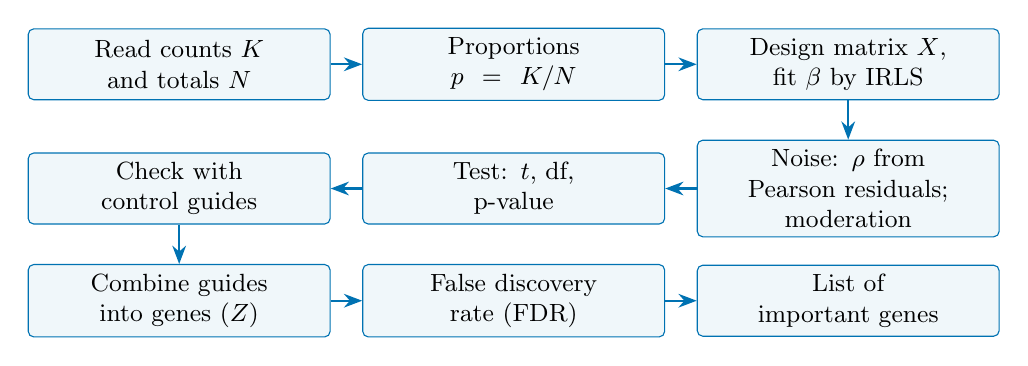
\begin{tikzpicture}[node distance=5mm and 4mm,
  box/.style={draw=barcsblue,fill=barcsblue!6,rounded corners=2pt,
              align=center,minimum height=9mm,text width=3.6cm,font=\small},
  arr/.style={-{Stealth},thick,barcsblue}]
\node[box] (a) {Read counts $K$\\and totals $N$};
\node[box,right=of a] (b) {Proportions\\$p = K/N$};
\node[box,right=of b] (c) {Design matrix $X$,\\fit $\beta$ by IRLS};
\node[box,below=of c] (d) {Noise: $\rho$ from\\Pearson residuals;\\moderation};
\node[box,left=of d] (e) {Test: $t$, df,\\p-value};
\node[box,left=of e] (f) {Check with\\control guides};
\node[box,below=of f] (g) {Combine guides\\into genes ($Z$)};
\node[box,right=of g] (h) {False discovery\\rate (FDR)};
\node[box,right=of h] (i) {List of\\important genes};
\draw[arr] (a)--(b); \draw[arr] (b)--(c); \draw[arr] (c)--(d);
\draw[arr] (d)--(e); \draw[arr] (e)--(f); \draw[arr] (f)--(g);
\draw[arr] (g)--(h); \draw[arr] (h)--(i);
\end{tikzpicture}
\end{center}

\subsection*{All symbols in one table}

\begin{center}
\small
\begin{tabular}{@{}l p{6.3cm} l@{}}
\toprule
Symbol & Meaning & Value in our example\\
\midrule
$K$ & read count of the guide in one library & 180, 240, 120, 80\\
$N$ & total read count of one library & 1.0, 1.2, 1.0, 0.8 million\\
$p$ & proportion, $K/N$ & 191 and 111 per million\\
fold change & $p_{\text{drug}} \div p_{\text{control}}$ & 0.58\\
$\log_2$ & number of doublings & $\log_2(0.58) = -0.78$\\
$\ln$ & natural logarithm (powers of $e = 2.718$) & $\ln(0.58) = -0.54$\\
log-odds & $\ln\bigl(p/(1-p)\bigr)$ & $-8.56$ (control)\\
$\mu$ & expected proportion & 0.000191 (control)\\
$\rho$ & biological noise & 0.000000386\\
$X$ & design matrix: a row per library, a column per $\beta$ & 4 rows, 2 columns\\
$\beta_0$ & control log-odds in the model & $-8.565$\\
$\beta_1$ & effect of the drug & $-0.542$\\
$\eta$ & predicted log-odds of a library (row of $X$ times $\beta$) & $-8.565$, $-9.107$\\
$w$ & weight of a library in the fit & 137.5 (library 1)\\
working value & prediction plus correction (Example 10) & $-8.621$ (library 1)\\
Pearson residual & distance from the prediction in SDs & $-0.65$ (library 1)\\
inflation & noise compared with counting noise & 1.376\\
SE & standard error of the effect & 0.101\\
$t$ & effect divided by SE & $-5.38$\\
df & libraries minus $\beta$ values & $4 - 2 = 2$\\
$p$-value & chance of this result if the effect is 0 & 0.033\\
$d_0$ & prior degrees of freedom (votes) & 12 (Example 15)\\
$z$, $Z$ & z score of a guide, of a gene & 3.46 (Example 18)\\
$m$ & number of guides for a gene & 3\\
$r$ & guide correlation (shared noise) & 0.1 (Example 19)\\
FDR & expected fraction of false hits & 0.005 for gene A\\
\bottomrule
\end{tabular}
\end{center}

Note: the letter $p$ has two uses in this guide. Alone, $p$ is a proportion.
In the word ``p-value'', it is a probability. The text always tells you
which one it is.

\newpage
%=====================================================================
\section{Quiz}
%=====================================================================

Choose the best answer. The answers and calculations are in the next
section.

\begin{enumerate}[label=\textbf{Q\arabic*.},leftmargin=2.6em,itemsep=6pt]

\item What does one guide do in a CRISPR screen?
\begin{choices}
\item It counts the cells.
\item It adds a drug to the cells.
\item It reads the DNA.
\item It switches off one gene.
\end{choices}

\item A library has $K = 300$ and $N = 1{,}500{,}000$. What is the count per
million?
\begin{choices}
\item 200
\item 300
\item 450
\item 500
\end{choices}

\item Why do we divide each count by its library total $N$?
\begin{choices}
\item To make the numbers bigger.
\item Because the machine reads some libraries more than others.
\item To remove the biological noise.
\item Because BARCS cannot use whole numbers.
\end{choices}

\item A guide has 400 per million in control and 100 per million with a
drug. What is the fold change?
\begin{choices}
\item 4
\item 0.4
\item 0.25
\item 300
\end{choices}

\item What is $\log_2(8)$?
\begin{choices}
\item 2
\item 3
\item 4
\item 8
\end{choices}

\item A gene has $\log_2(\text{fold change}) = -1$. What happened to its
guide?
\begin{choices}
\item It doubled.
\item It did not change.
\item It dropped to half.
\item It dropped to zero.
\end{choices}

\item For a very small proportion $p$, which statement is true?
\begin{choices}
\item The odds are almost equal to $p$.
\item The odds are almost equal to 1.
\item The odds are twice $p$.
\item The odds are always 0.
\end{choices}

\item In the variance formula, what does $\rho = 0$ mean?
\begin{choices}
\item There is no noise at all.
\item There is only counting noise.
\item There is only biological noise.
\item The guide has zero reads.
\end{choices}

\item Use $N\mu(1-\mu)$ with $N = 100$ and $\mu = 0.5$. What is the counting
variance?
\begin{choices}
\item 25
\item 50
\item 0.25
\item 100
\end{choices}

\item The machine reads each library ten times more deeply. What happens to
the biological noise?
\begin{choices}
\item It disappears.
\item It becomes ten times smaller.
\item It does not go away. Only more replicates help.
\item It becomes zero for control guides.
\end{choices}

\item In the design matrix of our example, which $\beta$ belongs to the
column of 1s?
\begin{choices}
\item $\beta_1$
\item the interaction
\item $\beta_0$
\item $\rho$
\end{choices}

\item BARCS gives $\beta_1 = 0.69$ for a guide. Use $e^{0.69} = 2.0$. What
does this mean?
\begin{choices}
\item The guide halves with the drug.
\item The guide does not change.
\item The guide disappears.
\item The guide doubles with the drug.
\end{choices}

\item An experiment has 6 libraries. The model has 3 $\beta$ values. How many
degrees of freedom does it have?
\begin{choices}
\item 3
\item 2
\item 6
\item 9
\end{choices}

\item An effect is $\beta_1 = -0.8$ with $\text{SE} = 0.2$. What is the $t$
value?
\begin{choices}
\item $-0.16$
\item $-1.0$
\item $-0.6$
\item $-4.0$
\end{choices}

\item A guide has df $= 2$ and its own noise 5.0. The typical noise is 2.0
with $d_0 = 8$. What is the moderated noise?
\begin{choices}
\item 2.0
\item 3.5
\item 5.0
\item 2.6
\end{choices}

\item A screen has 200 control guides. About how many should get $p < 0.05$
by chance?
\begin{choices}
\item 0
\item 5
\item 10
\item 50
\end{choices}

\item A gene has 4 guides, each with $z = 1.0$. What is $Z_{\text{gene}}$
(no shared noise)?
\begin{choices}
\item 1.0
\item 2.0
\item 4.0
\item 0.5
\end{choices}

\item Three genes have p-values 0.01, 0.02 and 0.30. What is the
Benjamini--Hochberg value $p \times 3 \div \text{rank}$ for the second gene?
\begin{choices}
\item 0.02
\item 0.06
\item 0.30
\item 0.03
\end{choices}

\item Why does BARCS 0.2.1 add a very small number to the counts of some
guides?
\begin{choices}
\item Because $\ln(0)$ does not exist when a group has zero reads.
\item To make all guides look important.
\item To increase the library totals.
\item To remove control guides.
\end{choices}

\item Which action gives BARCS more information about biological noise?
\begin{choices}
\item Read each library more deeply.
\item Use fewer guides.
\item Add more replicate libraries.
\item Use a larger p-value limit.
\end{choices}


\item An experiment has 3 control libraries and 3 drug libraries. The
formula is \texttt{\textasciitilde\ group}. What is the size of the design
matrix?
\begin{choices}
\item 3 rows and 2 columns
\item 6 rows and 2 columns
\item 2 rows and 6 columns
\item 6 rows and 3 columns
\end{choices}

\item A library has the row $(1, 1)$ in the design matrix. The values are
$\beta_0 = -8.0$ and $\beta_1 = -0.5$. What is the predicted log-odds?
\begin{choices}
\item $-8.5$
\item $-8.0$
\item $-7.5$
\item $4.0$
\end{choices}

\item In the knockout-and-drug design, which group has a 1 in the
interaction column?
\begin{choices}
\item normal, no drug
\item knockout, no drug
\item normal, drug
\item knockout, drug
\end{choices}

\item Two control libraries have weights 100 and 300. Their working values
are $-8.0$ and $-9.0$. What is the weighted average?
\begin{choices}
\item $-8.5$
\item $-8.25$
\item $-8.75$
\item $-9.0$
\end{choices}

\item The control weights add up to $W_{\text{control}} = 100$. The drug
weights add up to $W_{\text{drug}} = 25$. What is $\text{SE}(\beta_1)$?
\begin{choices}
\item 0.05
\item 0.224
\item 0.5
\item 1.25
\end{choices}

\item At $\rho = 0$, the squared Pearson residuals of a guide add up to 1.5.
The model has 2 degrees of freedom. Which $\rho$ does BARCS use?
\begin{choices}
\item $\rho = 0$
\item $\rho = 1.5$
\item $\rho = 0.75$
\item $\rho = 2$
\end{choices}

\item You add a paired-replicate column to the model of our four libraries.
How many degrees of freedom stay?
\begin{choices}
\item 3
\item 2
\item 4
\item 1
\end{choices}

\item Of 100 control guides, 95 have $|t|$ below 2.94. The $t$ table says
1.96. What is the scale factor?
\begin{choices}
\item 0.67
\item 1.0
\item 1.5
\item 4.9
\end{choices}
\end{enumerate}

\newpage
%=====================================================================
\section{Answers and calculations}
%=====================================================================

\begin{enumerate}[label=\textbf{Q\arabic*.},leftmargin=2.6em,itemsep=6pt]
\item \textbf{D.} Each guide switches off one gene (Section~1).
\item \textbf{A.} $300 \div 1{,}500{,}000 = 0.0002$. Then
  $0.0002 \times 1{,}000{,}000 = 200$ per million.
\item \textbf{B.} Libraries get different numbers of reads. Division by $N$
  makes them comparable (Step~1).
\item \textbf{C.} $100 \div 400 = 0.25$. The guide keeps one quarter of its
  control level.
\item \textbf{B.} $2 \times 2 \times 2 = 8$. You double three times, so
  $\log_2(8) = 3$.
\item \textbf{C.} $-1$ means one halving (Step~2).
\item \textbf{A.} $1 - p$ is almost 1, so $p/(1-p)$ is almost $p$
  (Step~3).
\item \textbf{B.} The extra factor becomes $1 + (N-1) \times 0 = 1$. Only
  counting noise stays (Step~4).
\item \textbf{A.} $100 \times 0.5 \times (1 - 0.5) = 100 \times 0.5 \times
  0.5 = 25$.
\item \textbf{C.} The factor $1 + (N-1)\rho$ grows with $N$. Deeper reading
  does not remove biological noise (Step~4).
\item \textbf{C.} The column of 1s is the intercept. It belongs to
  $\beta_0$, the starting level (Step~5).
\item \textbf{D.} The fold change is $e^{0.69} = 2.0$. The guide doubles.
\item \textbf{A.} $\text{df} = 6 - 3 = 3$ (Step~8).
\item \textbf{D.} $t = -0.8 \div 0.2 = -4.0$.
\item \textbf{D.} $(2 \times 5.0 + 8 \times 2.0) \div (2 + 8) = (10 + 16)
  \div 10 = 26 \div 10 = 2.6$ (Step~9).
\item \textbf{C.} $5\% \text{ of } 200 = 0.05 \times 200 = 10$ (Step~10).
\item \textbf{B.} $(1.0+1.0+1.0+1.0) \div \sqrt{4} = 4.0 \div 2 = 2.0$
  (Step~11).
\item \textbf{D.} The second gene has rank 2. So
  $0.02 \times 3 \div 2 = 0.03$ (Step~12).
\item \textbf{A.} With zero reads, the log-odds is $\ln(0)$, which does not
  exist. The Firth correction fixes this problem.
\item \textbf{C.} Degrees of freedom come from libraries. Only more
  replicates add information about biological noise (Steps~4 and~8).

\item \textbf{B.} One row for each library ($3 + 3 = 6$). One column for the
  intercept and one for drug (Step~5).
\item \textbf{A.} $1 \times (-8.0) + 1 \times (-0.5) = -8.5$ (Step~5).
\item \textbf{D.} The interaction column is knockout times drug. Only
  $1 \times 1 = 1$ (Step~5).
\item \textbf{C.} $(100 \times (-8.0) + 300 \times (-9.0)) \div (100 + 300)
  = (-800 - 2700) \div 400 = -3500 \div 400 = -8.75$ (Step~6).
\item \textbf{B.} $\sqrt{1/100 + 1/25} = \sqrt{0.01 + 0.04} = \sqrt{0.05}
  = 0.224$ (Step~8).
\item \textbf{A.} The sum (1.5) is already 2 or less. So BARCS uses
  $\rho = 0$ (Step~7).
\item \textbf{D.} The model now has 3 columns. So
  $\text{df} = 4 - 3 = 1$ (Step~5).
\item \textbf{C.} $2.94 \div 1.96 = 1.5$ (Step~10).
\end{enumerate}

\end{document}
